\documentclass[a4paper]{article}

%\VignetteIndexEntry{Introduction to ggcluster}
%\VignettePackage{ggcluster}

% Definitions
%\newcommand{\slan}{{\tt S}}
%\newcommand{\rlan}{{\tt R}}
\newcommand{\ggcluster}{{\tt ggcluster}}
\newcommand{\clusterdata}{\code{cluster\_data}}
\newcommand{\code}[1]{{\tt #1}}
\setlength{\parindent}{0in}
\setlength{\parskip}{.1in}
\setlength{\textwidth}{140mm}
\setlength{\oddsidemargin}{10mm}

\title{Introduction to the \ggcluster{} package for plotting cluster analysis results}
\author{Andrie de Vries}

\usepackage{Sweave}
\begin{document}

\maketitle

\ggcluster{} is a package that makes it easy to extract results of cluster analysis into a data frame.  It provides a common framework for a number of hierarchical and other cluster analysis techniques, including:
\itemize{
\item hclust() - hierarchical clustering
\item dendrogram()- dendrograms
\item kmeans() - k-means clustering
\item Mclust() - model based clustering
}

\section{Introduction}

Most of the cluster analysis functions in R, e.g. \code{hclust()} and \code{dendrogram()} provide \code{plot()} functions to display the results.  However, it is sometimes hard to extract the data from this analysis to customise these plots, especially when the \code{plot()} functions don't provide an option to return the data.

The \ggluster{} package provides a general framework to extract the plot data for a variety of cluster analysis functions.

It does this by providing generic function \clusterdata{} that will extract the appropriate cluster data as well as labels.  This data is returned as a list of data.frames.  These data frames can 
  
\begin{Schunk}
\begin{Sinput}
> library(ggplot2)
> library(ggcluster)
\end{Sinput}
\end{Schunk}


\section{Dendrograms}

The \code{hclust()} and \code{dendrogram()} functions in R makes it easy to plot the results of hierarchical cluster analysis and other dendrograms in R.  However, it is hard to extract the data from this analysis to customise these plots, since the \code{plot()} functions for both these classes prints directly without the option of returning the plot data.  

\begin{Schunk}
\begin{Sinput}
> hc <- hclust(dist(USArrests), "ave")
> dhc <- as.dendrogram(hc)
> ddata <- cluster_data(dhc, type = "rectangle")
> p <- ggplot(ddata$segments) + geom_segment(aes(x = x0, y = y0, 
+     xend = x1, yend = y1)) + coord_flip() + scale_y_reverse(expand = c(0.2, 
+     0))
> print(p)
\end{Sinput}
\end{Schunk}

\begin{figure}[h]
\begin{center}
{
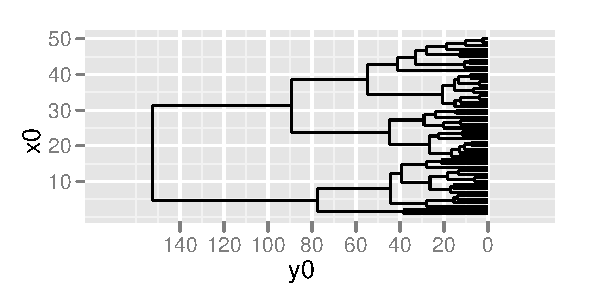
\includegraphics[width=4in, height=2in]{ggcluster-dendro1}
}
\end{center}
\caption{A dendrogram produced using \clusterdata{} and \code{ggplot()}}
\end{figure}


Of course, using ggplot to create the dendrogram means one has full control over the appearance of the plot.  For example, here is the same data, but this time plotted horizontally with a clean background:

\begin{Schunk}
\begin{Sinput}
> p <- p + coord_flip() + opts(panel.grid.major = theme_blank(), 
+     panel.grid.minor = theme_blank(), panel.background = theme_blank(), 
+     axis.title.x = theme_text(colour = NA), axis.title.y = theme_blank(), 
+     axis.text.x = theme_blank(), axis.text.y = theme_blank(), 
+     axis.line = theme_blank())
> print(p)
\end{Sinput}
\end{Schunk}

\begin{figure}[h]
\begin{center}
{
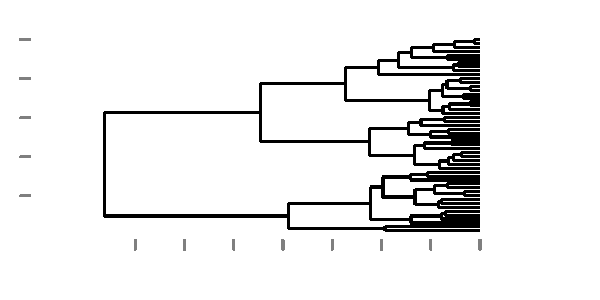
\includegraphics[width=4in, height=2in]{ggcluster-dendro2}
}
\end{center}
\caption{Dendrogram rotated on clear background}
\end{figure}

Dendrograms can also be drawn using triangular lines instead of rectangular lines.  For example:

\begin{Schunk}
\begin{Sinput}
> ddata <- cluster_data(dhc, type = "triangle")
> p <- ggplot(ddata$segments) + geom_segment(aes(x = x0, y = y0, 
+     xend = x1, yend = y1)) + coord_flip() + scale_y_reverse(expand = c(0.2, 
+     0)) + opts(panel.grid.major = theme_blank(), panel.grid.minor = theme_blank(), 
+     panel.background = theme_blank(), axis.title.x = theme_text(colour = NA), 
+     axis.title.y = theme_blank(), axis.text.x = theme_blank(), 
+     axis.text.y = theme_blank(), axis.line = theme_blank())
> print(p)
\end{Sinput}
\end{Schunk}

\begin{figure}[h]
\begin{center}
{
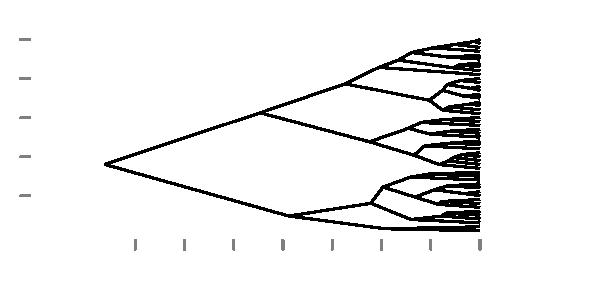
\includegraphics[width=4in, height=2in]{ggcluster-dendro3}
}
\end{center}
\caption{A dendrogram with triangular connection lines}
\end{figure}

  

\section{Tree diagrams}

\ggcluster{} can also deal with tree plots.

\begin{Schunk}
\begin{Sinput}
> data(cpus, package = "MASS")
> cpus.ltr <- tree(log10(perf) ~ syct + mmin + mmax + cach + chmin + 
+     chmax, cpus)
> tree_data <- cluster_data(cpus.ltr)
> p <- ggplot(tree_data$segments) + geom_segment(aes(x = x, y = y, 
+     xend = xend, yend = yend, size = n), colour = "blue", alpha = 0.5) + 
+     scale_size("n", to = c(0, 3)) + geom_text(data = tree_data$labels, 
+     aes(x = x, y = y, label = label), vjust = -0.5, size = 4) + 
+     geom_text(data = tree_data$leaf_labels, aes(x = x, y = y, 
+         label = label), vjust = 0.5, size = 3)
> print(p)
\end{Sinput}
\end{Schunk}

\begin{figure}[h]
\begin{center}
{
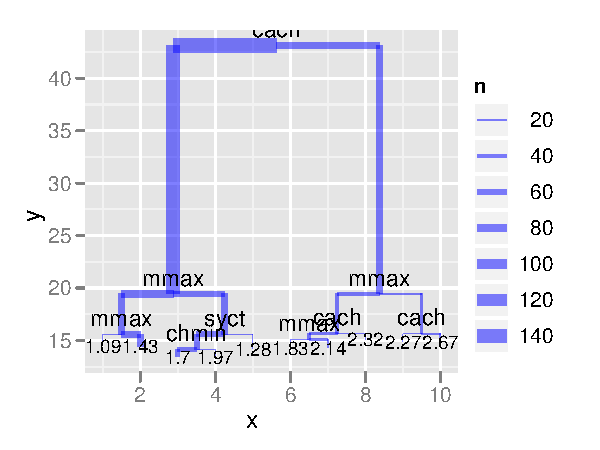
\includegraphics[width=4in, height=3in]{ggcluster-tree1}
}
\end{center}
\caption{Tree plot}
\end{figure}


\section{Cluster analysis}

Some text here.

\section{Final thoughts}

The last word.


% Start a new page
% Not echoed, not evaluated
% ONLY here for checkVignettes so that all output doesn't
% end up on one enormous page

\end{document}




